\documentclass[9pt, aspectratio=169]{beamer}

\usetheme[progressbar=frametitle]{metropolis}
\definecolor{lightgray}{RGB}{50, 60, 60}
\definecolor{pitchblack}{RGB}{0, 0, 0}
\definecolor{lightbeige}{RGB}{255, 251, 241}
\definecolor{mediumgray}{RGB}{200, 200, 200}

\setbeamercolor{background canvas}{bg=white}
%\setbeamercolor{normal text}{fg=lightbeige}
%\setbeamercolor{frametitle}{bg=lightgray, fg=mediumgray}

%\setbeamertemplate{blocks}[rounded][shadow]

%\setbeamercolor{block title}{fg=white,bg=blue!70}
%\setbeamercolor{block body}{bg=blue!20}

\usepackage[utf8]{inputenc}
\graphicspath{{images/}{images/theme/}}
	
\usepackage{tabularx}	
\setbeamertemplate{caption}[numbered]
\setbeamertemplate{footline}[frame number]
\usepackage{algorithm}
\usepackage{algorithmic}
	
\usepackage{amsmath} % assumes amsmath package installed
\usepackage{amssymb}  % assumes amsmath package installed
\usepackage[mathcal]{euscript}
\usepackage{pifont}% http://ctan.org/pkg/pifont
%\usepackage{hyperref}
\usepackage{multirow}
%\hypersetup{colorlinks=true}
\newcommand{\cmark}{\ding{51}}%
\newcommand{\xmark}{\ding{55}}%

\usepackage{bm}
%\usepackage{natbib} %Apa style for citation
\usepackage{bibentry}
\nobibliography*

\newcommand{\footfullcite}[1]{\footnote{\scriptsize{\bibentry{#1}}}}

%% DONNES UTILES A LA PAGE DE TITRE ET AU PIED DE PAGE...
\title{Geometric Camera Pose Refinement with Learned Depth Maps}
%\subtitle{Localisation basée image en conditions difficiles par apprentissage de modalités}
\author{\textbf{Nathan Piasco$^{1,2}$}, Désiré Sidibé$^{1}$, Valérie Gouet-Brunet$^{2}$ and Cédric Demonceaux$^{1}$}
\institute{pLaTINUM metting, Paris} % ON SE SERT DE INSTITUTE POUR METTER LE LIEUX DE LA CONF
\date{04/06/2019}

%\definecolor{IGNVert}{RGB}{148, 192,  22}
%\definecolor{IGNGris}{RGB}{112, 119, 122}
%\definecolor{IGNRouge}{RGB}{255, 100, 100}
\usepackage{ragged2e}
\newcommand{\norm}[1]{\left\lVert#1\right\rVert}
\newcommand{\abs}[1]{\left\lvert#1\right\rvert}

\begin{document}

\begin{frame}[plain,c]
	\titlepage
	\begin{minipage}{0.49\textwidth}
	\footnotesize
	\centering
		\begin{enumerate}
			\item VIBOT ERL,CNRS  6000,  ImViA, Universit\'e  Bourgogne Franche-Comt\'e
			\item LaSTIG, IGN, ENSG, Universit\'e Paris-Est, 	F-94160 Saint-Mand\'e, France
		\end{enumerate}
	\end{minipage}\hfill
	\begin{minipage}{0.49\textwidth}
	\centering
	{
	\begin{minipage}{0.45\linewidth}
			\centering
			\includegraphics[width=0.5\linewidth]{images/logos/ign_logo}
	\end{minipage}\hfill
	\begin{minipage}{0.45\linewidth}
			\centering
			\includegraphics[width=0.5\linewidth]{images/logos/cnrs}
	\end{minipage}

	\vfill
	
	\begin{minipage}{0.45\linewidth}
			\centering
			\includegraphics[width=0.7\linewidth]{images/logos/ubfc}
	\end{minipage}\hfill
	\begin{minipage}{0.45\linewidth}
			\centering
			\includegraphics[width=0.5\linewidth]{images/logos/vibot}	
	\end{minipage}
	}
%	\begin{tabular}{c c}
%		\includegraphics[width=0.19\linewidth]{images/logos/ign_logo} & 
%			\includegraphics[width=0.15\linewidth]{images/logos/cnrs} \\
%					\includegraphics[width=0.27\linewidth]{images/logos/ubfc} &
%							\includegraphics[width=0.23\linewidth]{images/logos/vibot} \\
%	\end{tabular}
	\end{minipage}
\end{frame}

\section{Introduction}

\label{sec:intro}

\begin{frame}{Problem statement}
	\begin{minipage}{0.47\linewidth}
		\centering
		\begin{figure}
			\includegraphics[width=0.55\linewidth]{images/intro/patchwork/nn_candidat}
		\end{figure}	
		Unknown pose \textcolor<2>{red}{query image}.
		
		\vfill
		
		\begin{figure}
			\includegraphics[width=0.7\linewidth]{images/intro/patchwork/patchwork}
		\end{figure}	
		\textcolor<2>{green}{Reference dataset images.}
	\end{minipage}\hfill
	\begin{minipage}{0.5\linewidth}
		\centering
		\uncover<2->
		{
		\begin{figure}
			\includegraphics[width=0.6\linewidth]{images/intro/heads}
		\end{figure}	
		}	
		
		\vfill		
		
		\only<1>{
			\huge
			Original image localization problem casted as an image retrieval task.
		}
		\only<2>{
			\huge
			References images do not cover the entire scene.
		}	
		 \only<3>{
			\huge
			Solution: pose refinement.
		}
	\end{minipage}
	
\end{frame}

\begin{frame}{Pose estimation methods}
	\begin{itemize}
		\item 2D features to 3D point cloud matching\footfullcite{Sattler2016a}
		\item<2-> Coarse to find\footfullcite{Taira2018}
		\item<3-> Learned methods\footfullcite{Brachmann2017a}
	\end{itemize}
		
	\vfill	
	
	\only<1>
	{
		\textcolor{blue}{Fast and precise} but \textcolor{red}{requires a sparse 3D model of the environment}.
	}
	\only<2>
	{
		\textcolor{blue}{Scalable and robust} but \textcolor{red}{uses two steps to compute the real pose}.
	}
	\only<3>
	{
		\textcolor{blue}{Compact and provide direct absolute pose} but \textcolor{red}{needs a specific CNN training for each scene}.
	}
		
\end{frame}	

\begin{frame}{Our idea}
		\begin{figure}
			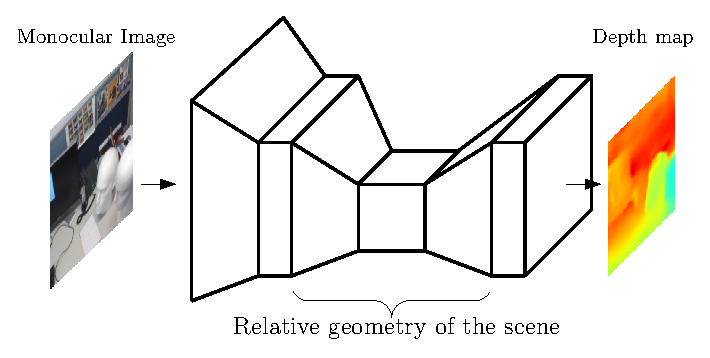
\includegraphics[width=0.5\linewidth]{images/intro/encoder_dec}
		\end{figure}	
		
		\vfill
		
		We learn the relative geometry of the scene to refine the query position and orientation.
\end{frame}


\section{Pose Refinement with Learned Depth Maps}

\label{sec:method}

\begin{frame}{Method overview}
	\only<1>{
		\begin{figure}
		\centering		
		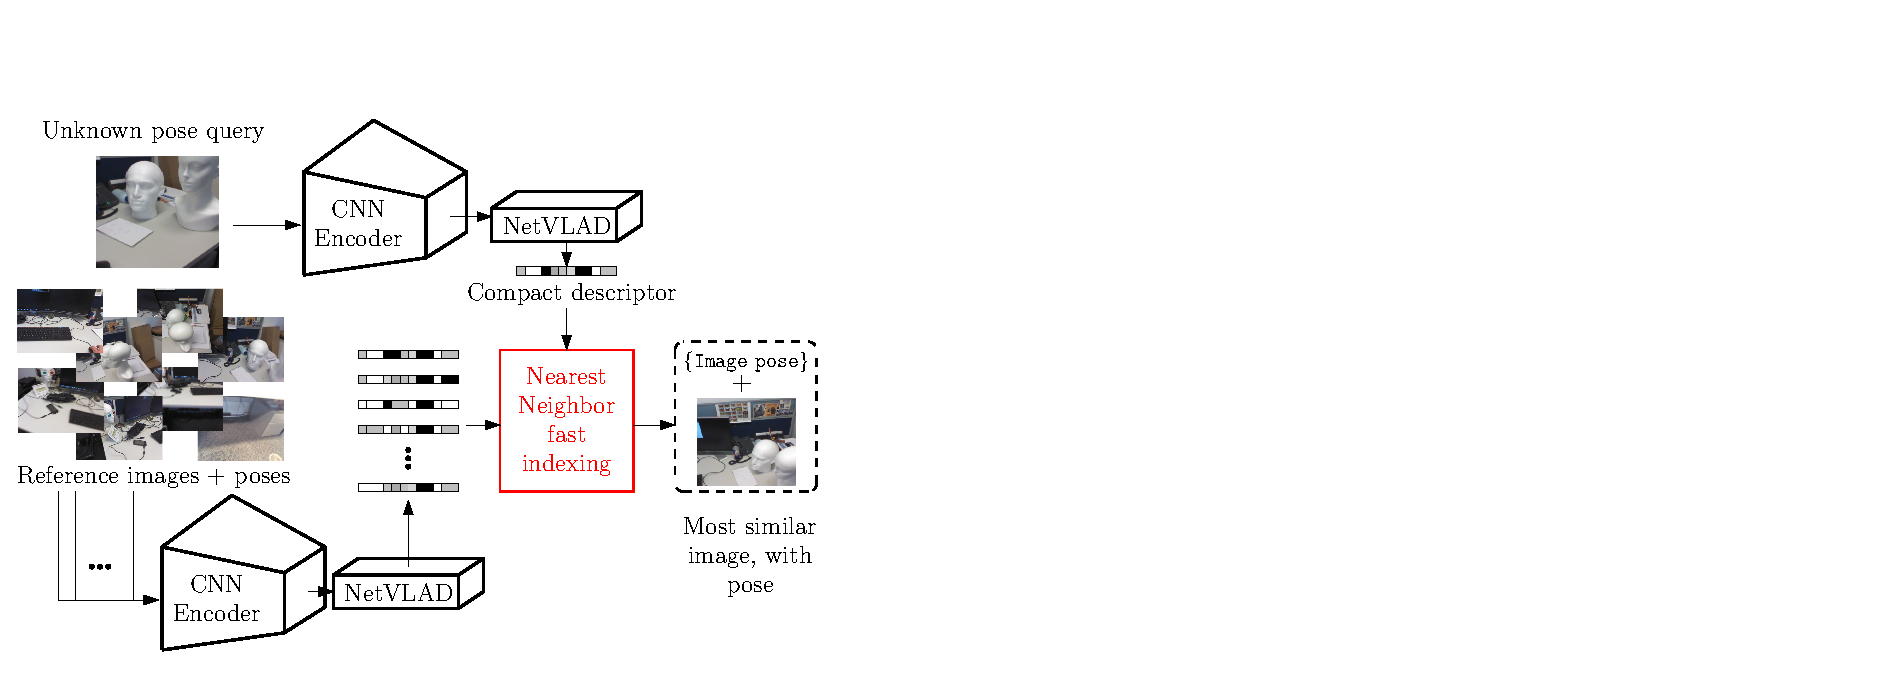
\includegraphics[width=0.9\linewidth]{images/method/1}
		\end{figure}
		
		\vfill
		
		Initial pose obtained by image retrieval.
	}
	\only<2>
	{
		\begin{figure}
		\centering
		\includegraphics[width=0.9\linewidth]{images/method/2}
		\end{figure}	
		
		\vfill
		
		Dense correspondences are made by matching CNN deep features.
	}
	\only<3>
	{
		\begin{figure}
		\centering
		\includegraphics[width=0.9\linewidth]{images/method/3}
		\end{figure}	
		
		\vfill
	
		\textbf{Method 1)} Initial approach: projection of the matched 2D points according to the produced depth map and alignment of the obtained 3D points clouds by ICP.
	}
	\only<4>
	{
		\begin{figure}
		\centering
		\includegraphics[width=0.9\linewidth]{images/method/4}
		\end{figure}	
		
		\vfill
	
		\textbf{Method 2)} Minimising the depth incertitude: pose estimation by Perspective-n-Point (PnlP).
	}
\end{frame}

\begin{frame}{Method details}
	Dense local correspondences:
	\begin{itemize}
		\item feature block with same spatial dimension as depth output (2nd conv. block)
		\item bidirectional matching
	\end{itemize}

	\vfill	
	
	\uncover<2>
	{
	Pose estimation:
	\begin{itemize}
		\item ICP and PnP optimization within RANSAC
		\item we evaluate the top 5 retrieved candidates from the image retrieval first step
	\end{itemize}
	}
\end{frame}

\begin{frame}{System design and motivation}
	\begin{block}{Multi-task model}
		Same network for: global image description, dense local feature matching and depth from monocular.
	\end{block}
	\vfill
	\uncover<2->
	{
		\begin{block}{Single task training policy}
			We decide to train our network for the task of depth from monocular because erroneous depth estimation measurement will result in wrong estimation of the final pose.
		\end{block}
	}
	\vfill
	\uncover<3>
	{
		\begin{block}{Generalisation}
			The same trained network can be used to localise images in multiple indoor and outdoor scenes, and even on totally unknown environments.
		\end{block}
	}
\end{frame}


\section{Experiments}

\label{sec:results}

\begin{frame}{Datasets \& training}
	Depth from monocular training:
	\begin{itemize}
		\item \textbf{sup} supervised training (images + depth maps)
		\item \textbf{unsup} unsupervised training (image sequence + relative pose)\footfullcite{Zhou2017a}
	\end{itemize}
	\uncover<2>
	{
		Indoor datasets:
		\begin{itemize}
			\item 7 scenes\footfullcite{Shotton2013}
			\item 12 scenes\footfullcite{Valentin2016} (generalization)
		\end{itemize}
		Outdoor dataset:
		\begin{itemize}
			\item Cambridge landmarks\footfullcite{Kendall2015}
		\end{itemize}
	}

\end{frame}

\begin{frame}{ICP vs. PnlP}
	\centering
	\input{tabs/icp/7_scenes_results}
	
	\vfill
	
	Initial results for 7 scenes indoor dataset.
\end{frame}

\begin{frame}{PnlP -- Indoor results}
	\centering
	\input{tabs/pnlp/7_scenes}
	
	\vfill
	
	Comparison between supervised and unsupervised training.
\end{frame}

\begin{frame}{PnlP -- Indoor generalization}
	\centering
	\input{tabs/pnlp/12_scenes}
	
	\vfill
	
	Generalization on unseen scene.
\end{frame}

\begin{frame}{Depth maps}
	\begin{figure}
		\includegraphics[width=\linewidth]{images/results/depth_map/fig1/fig1-noborder}
	\end{figure}
\end{frame}

\begin{frame}{PnlP -- Outdoor}
	\centering
	\input{tabs/pnlp/outdoor}

	\vfill	
	
	\begin{figure}
		\includegraphics[width=\linewidth]{images/results/depth_map/fig2/fig2-wborder}
	\end{figure}

\end{frame}
\section{Conclusion}

\label{sec:conclusion}

\begin{frame}{Conclusion}
	Summary:
	\begin{itemize}
		\item 2-step pose estimation method, from coarse to find localization,
		\item use of the relative geometric information learned by CNN from raw RGB images to recover the real pose of the query,
		\item unlike learned approaches, the proposed method can be used in completely unknown environments.
	\end{itemize}

	\vfill
	
	\uncover<2->
	{
	For future works we want to find a common optimization framework to train each of the computer vision task involved in the pose refinement process.
	}
\end{frame}


%%%%%%%%%%%%%%%%%%%%%%%%%%%%%%%%%%%%%%%%%%%%%%%%%%%%%%%%%%%%%%%%%%%%%%%%%%%%%%%%%%%%%%%
% Biblio
\begin{frame}[plain, allowframebreaks]
\frametitle{References}
\bibliographystyle{alpha_c}
\scriptsize{\bibliography{bib/mendeley.bib}}

\end{frame}

\appendix

\end{document}
